\chapter{Изучение собственной и примесной фотопроводимости полупроводников}

\section{Цель работы}
Измерение спектра собственной и примесной фотопроводимости полупроводника. Определение ширины запрещённой зоны и энергии ионизации примеси. Исследование влияния поверхностной рекомбинации на форму спектра фотопроводимости.

\section{Теоретическая часть}
\subsection{Фотопроводимость}
При освещении полупроводника светом с достаточной энергией фотонов может возникнуть внутренний фотоэлектрический эффект, или иначе - фотопроводимость. Причиной появления  избыточной фотопроводимости может являться как увеличение концентрации свободных носителей заряда в результате оптической генерации, так и повышение подвижности в результате перехода носителей из подзоны с более тяжёлыми носителями в подзону более лёгких. Во втором случае общее количество носителей остаётся неизменным, но за счёт увеличения подвижности удельное электросопротивление материала падает. Этот эффект может наблюдаться при низких температурах.

В дальнейшем будем считать подвижность носителей постоянной, и рассматривать исключительно повышение проводимости материала за счёт изменения концентрации носителей. Это увеличение может быть связано с процессом фотоионизации атомов основного вещества или примеси, то есть, с собственным и примесным поглощением света в полупроводнике.

\subsection{Собственная и примесная фотопроводимость}
Оптическое излучение на собственной полосе поглощения полупроводника переводит валентные электроны в зону проводимости, то есть, приводит к генерации избыточных электронов в зоне проводимости и дырок в валентной зоне в равных соотношениях, если отсутствует захват преимущественный захват электронов или дырок ловушками.
Изменение проводимости полупроводника под действием освещения собственным светом описывается избыточной фотопроводимостью $\Delta \sigma$, определяемый как разница между величинами удельной электропроводности в освещённом и затемнённом состояниях:

\begin{equation}
\Delta \sigma = \sigma - \sigma_{\text{т}} = e (\mu_{n} \Delta n + \mu_{p} \Delta p).
\end{equation}

В широкозонных полупроводниках при комнатной температуре собственная концентрация носителей очень мала, и поэтому избыточная фотопроводимости может на порядки превышать темновую. В узкозонных ($E_{g} \le 1 \text{эВ}$) наоборот концентрация избыточных носителей мала по сравнению с собственной, и поэтому практически всегда реализуется условие малого уровня инжекции.

Длинноволновая граница собственной фотопроводимости совпадает с краем собственного поглощения и для узкозонных полупроводников лежит в инфракрасной области спектра. Для широкозонных полупроводников она может лежать в синей или даже ультрафиолетовой области. Связь между пороговой длиной волны и шириной запрещённой зоны для случая собственной фотопроводимости определяется известным соотношением:

\begin{equation}
\lambda_{\text{гр}} = \frac{h c}{E_{g}} = \frac{1240}{E_{g}}
\end{equation}
где $E_{g}$ выражается в электрон-вольтах, а $\lambda_{\text{гр}}$ - в нанометрах.

При фотоионизации примесей возрастает концентрация электронов в зоне проводимости или дырок в валентной зоне. При этом происходят переходы между уровнями примеси внутри запрещённой зоны и разрешёнными зонами. Такая фотопроводимости называется примесной.

\subsection{Спектральная зависимость фотопроводимости}
В общем случае отношение фотопроводимости к интенсивности падающего света - так называемая фоточувствительность - зависит от длины волны. Для анализа спектра фотопроводимости рассмотрим уравнение непрерывности:

\begin{equation}
\frac{\partial (\Delta n)}{\partial t} = \frac{1}{e} div \overrightarrow{j_{n}} + G_{n} - \frac{\Delta n}{\tau_{n}}
\end{equation}
для электронов.

Если мы рассмотрим полупроводник в отсутствии электрического тока, то в стационарном состоянии уравнение имеет решение:

\begin{equation}
\Delta n = G_{n} \tau_{n}
\end{equation}

А для фотопроводимости можно записать

\begin{equation}
\Delta \sigma = q (\mu_{n} G_{n} \tau_{n} + \mu_{p} G_{p} \tau_{p})
\end{equation}

Так как величина $G_{n}$ зависит от интенсивности падающего излучения $I$ и коэффициента поглощения на данной длине волны $\alpha(\lambda)$, то и фотопроводимость будет определяться этими величинами. Для случая малого уровня инжекции зависимость времени жизни от концентрации носителей можно считать пренебрежимо малой.

Пусть на полупроводник толщиной $d$ падает свет с длиной волны $\lambda$, коэффициент поглощения на данной длине волны составляет $\alpha$. Тогда если образец достаточно тонкий, то есть, $\alpha d \ll 1$, то излучение равномерно поглощается по всему объёму образца, и избыточные носители заряда генерируются равномерно. Если $I$ - интенсивность падающего излучения, то энергия, поглощаемая в единице объёма образце будет равна $\alpha I$, а значит количество электрон-дырочных пар, генерируемых в единице объёма за единицу времени, равно $\eta \alpha I / h \nu$. Здесь $\eta$ - внутренний квантовый выход, то есть, вероятность того, что поглощённый фотон генерирует пару электрон-дырка.
Таким образом, скорость оптической генерации равна

\begin{equation}
G_{n} = \eta_{n} \frac{\alpha I}{h \nu} = \eta_{n} \alpha Q
\end{equation}
где $Q = I / h \nu$  - поток фотонов.

С учётом этого, можно записать спектральную зависимость фотопроводимости полупроводника:

\begin{equation}
\Delta \sigma = q (\eta_{n} \tau_{n} \mu_{n} + \eta_{p} \tau_{p} \mu_{p}) \alpha Q
\end{equation}

\subsection{Спектральная характеристика собственной фотопроводимости}
При равномерной генерации носителей и при отсутствии поверхностной рекомбинации, спектр собственной фотопроводимости определяется спектральной зависимостью коэффициента собственного поглощения. Например, для разрешённых прямых переходов коэффициент поглощения определяется формулой

\begin{equation}
\alpha(h \nu) = \frac{e^2 \left( 2 \frac{m_{n} m_{p}}{m_{n} + m_{p}} \right)^{3/2}}{\tilde{n} c h^2 m_{n}} \cdot (h \nu - E_{g})^{1/2}
\end{equation}

Собственная фотопроводимость при прямых переходах резко возрастает при энергии фотона $h \nu \ge E_{g}$, и при дальнейшем увеличении энергии практически не меняется.

Рассмотрим случай неравномерного поглощения, когда толщиной образца уже нельзя пренебречь. В таком случае

\begin{equation}
G_{y} = \frac{\alpha I_{0} (1-R)}{h \nu} \exp(-\alpha y)
\end{equation}

Будем считать, что толщина образца такова, что излучение практически не достигает дальней стенки образца. Тогда с ростом энергии фотона в основной полосе коэффициент поглощения увеличивается, а значит скорость генерации резко уменьшается по мере прохождения излучения вглубь образца. Из-за этого спектральная зависимость фотопроводимости с увеличением энергии фотонов проходит через максимум, а затем быстро уменьшается.

Учёт влияния поверхностной рекомбинации приводит к уменьшению концентрации вблизи поверхности образца. Если предполагать, что оптическое поглощение происходит равномерно по всему объёму, то единственным изменением, связанным с рекомбинацией на поверхности, будет замена величины $\tau$ на некоторое эффективное время жизни $\tau_{eff}$, зависящее как от времени жизни в объёме $\tau_{v}$, так и поверхностного времени жизни $\tau_{s} = \frac{d}{2 S} + \frac{d^2}{\pi^2 D}$, где $D$ - коэффициент диффузии, а $S$ - скорость поверхностной рекомбинации:

\begin{equation}
\frac{1}{\tau_{eff}} = \frac{1}{\tau_{v}} + \frac{1}{\tau_{s}}
\end{equation}

Это значит, что фотопроводимость при учёте поверхностной рекомбинации окажется в $\frac{\tau_{v}}{\tau_{eff}}$ раз меньше, чем было бы при $S = 0$. При этом поверхностная рекомбинация влияет не только на стационарное значение, но и на вид спектра фотопроводимости. Так, при измерении спектра фотопроводимости в основной полосе поглощения, где коэффициент поглощения сильно возрастает, сказываются два конкурирующих процесса: за счёт увеличения коэффициента поглощения увеличивается величина фотопроводимости, в то же время доля избыточной концентрации, генерируемая вблизи поверхности возрастает, а именно там поверхностные эффекты влияют наиболее заметно. Эти процессы приводят к тому, что в спектральной зависимости фотопроводимости будет наблюдаться максимум фотопроводимости вблизи края собственного поглощения, и чем больше величина $S$, тем сильнее будет выражен этот максимум. Структурные особенности спектра фотопроводимости с учётом влияния поверхностной рекомбинации приведёт на рисунке \ref{pic7_SR}, на нём же приведена кривая спектра поглощения (штрихпунктирная линия). Чтобы учесть этот эффект за длинноволновую границу собственной фотопроводимости принимается длина волны $\lambda_{\frac{1}{2}}$ на длинноволновом спаде спектральной характеристики, при которой фотопроводимость уменьшается в два раза по сравнению с максимальной.

\begin{figure}[h!]\centering
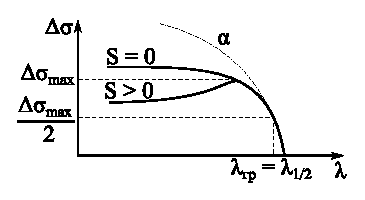
\includegraphics{pic7_SR.eps}
\caption{Спектр собственной фотопроводимости при отсутствии $(S = 0)$ и наличии $(S > 0)$ поверхностной рекомбинации}
\label{pic7_SR}
\end{figure}

\subsection{Спектральная характеристика примесной фотопроводимости}
В примесном кристалле оптические переходы электронов между локальными уровнями примесей (или других нарушений идеальности кристаллического поля) и главными энергетическими зонами приводят к появлению примесного поглощения и примесной фотопроводимости. Так как энергия ионизации мелких примесей лежит вблизи основных зон, то примесная фотопроводимость занимает на спектре область длин волн вблизи края собственной проводимости, а также имеет несколько полос в длинноволновой области, в зависимости от того, какой электронный переход примесь-зона имеет место.

Спектр примесной фотопроводимости достаточно хорошо совпадает со спектром примесного поглощения. Рассмотрим основные оптические переходы в полупроводнике, приводящие к фотопроводимости. Если мелкий уровень нейтрален, то под действием кванта излучения $h \nu \ge E_{i}$, где $E_{i}$  - энергия ионизации примеси, электрон из валентной зоны перейдёт на акцепторный уровень или с донорного уровня перейдёт в зону проводимости. Такие переходы сопровождаются поглощением в области длин волн между $\lambda_{i}$ и $\lambda_{\text{гр}}$. Здесь поглощение растёт с уменьшением длины волны и резко обрывается при $\lambda = \lambda_{\text{i}}$.

Если мелкий уровень ионизован, в области $\lambda \le \lambda_{\text{гр}}$ возникают полосы поглощения, связанные с переходами электронов из валентной зоны на уровень ионизованных доноров или с уровней ионизованных акцепторов в зону проводимости. На рисунке \ref{pic7_transition} показаны обе группы переходов: 1 и 2 - переходы с уровня ионизованного акцептора в зону проводимости, 3 и 4 - переход из валентной зоны на ионизованный донор. Энергия этих переходов близка к ширине запрещённой зоне, и поэтому полосы поглощения, связанные с этими переходами, образуют в длинноволновой части края собственного поглощения ступеньку. Цифрами 5 и 6 обозначены переходы электронов между мелким уровнем и ближней зоной. Энергия таких переходов много меньше ширины запрещённой зоны. Эти переходы заметны только при достаточно глубоком охлаждении полупроводника.

\begin{figure}[h!]\centering
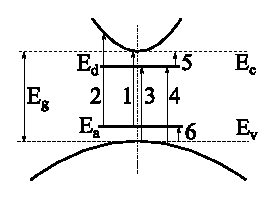
\includegraphics{pic7_transition.eps}
\caption{Схема возможных переходов в примесном кристалле}
\label{pic7_transition}
\end{figure}

В случае переходов 1, 2 и 5 в переносе заряда будут участвовать свободные электроны. Для переходов 3, 4 и 6 такими носителями являются дырки.

Рассмотрим схему оптического поглощения, связанного с переходами электронов с ионизованных акцепторов в зону проводимости. Интервал энергий фотона, соответствующий поглощению, определяется величиной вектора $\overrightarrow{k}_{a}$ волновой функции электрона на акцепторе. Величины волнового вектора, для которых волновые функции будут значительны, находятся в пределах обратного радиуса боровской орбиты акцепторного состояния. Поэтому область энергий с достаточно большим поглощением будет определяться границами:

\begin{equation}
E_{g} - E_{a} < h \nu < E_{g} - E_{a} + E_{c}(\overrightarrow{k}_{a})
\end{equation}

На рисунке \ref{pic7_transition} акцепторный уровень изображён в виде горизонтальной линии, длина которой в k-пространстве равна $|\overrightarrow{k}_{a}|$. Количественно спектр поглощения, связанный с переходами $E_{a} \rightarrow E_{c}$ представляется формулой:

\begin{equation}
\alpha = \frac{A N_{a}}{1+\exp \left[ \frac{E_{a} - F}{k T} \right]} \cdot \frac{h \nu - E_{g} + E_{A}}{h \nu}
\end{equation}
где $A$ - постоянный множитель, не зависящий от частоты, $N_{a}$ - концентрация акцепторных состояний, $F$ - уровень Ферми.

Спектр примесного поглощения имеет ту же зависимость от частоты, что и поглощение, связанное с разрешёнными прямыми межзонными переходами. Только величины поглощения значительно меньше основного и предшествуют основному по шкале энергий фотонов. Отличие также состоит в том, что поглощение зависит от концентрации акцепторных примесей $N_{a}$ и температуры.

Поглощение, вызванное переходами электронов с акцепторного уровня в зону проводимости, будет проявляться в виде широкой полосы и перекрываться с полосой собственного поглощения. Спектр примесной фотопроводимости в этом случае будет представлять собой ступеньку в длинноволновой части спектра (см. рисунок \ref{pic7_spectrum}). Энергия ионизации примеси определяется по положению точки на длинноволновом спаде, где примесная фотопроводимости составляет половину от максимального значения в примесной области поглощения. Значение энергии ионизации, определённое таким образом из спектра поглощения, находится в хорошем согласии со значениями $E_{i}$, полученными другими методами.

\begin{figure}[h!]\centering
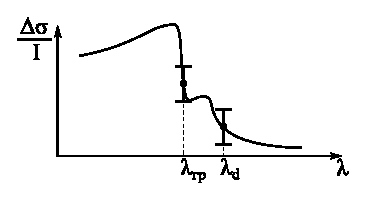
\includegraphics{pic7_spectrum.eps}
\caption{Спектры фотопроводимости примесного полупроводника при поглощении акцепторная примесь - зона проводимости}
\label{pic7_spectrum}
\end{figure}

\section{Методика измерений и описание установки}
Для определения спектра фотопроводимости необходимо знать зависимость фотопроводимости образца и интенсивности источника от длины волны. В данной работе в качестве образца используется фоторезистор, сопротивление которого измеряется при помощи универсального вольтметра В7-138. Чувствительность детектора очень велика, поэтому при измерении его необходимо затемнять.

Измерение спектра фоточувствительности можно проводить в относительных единицах, что позволит избежать трудоёмких измерений абсолютного значения интенсивности света. Для этого достаточно знать спектр относительной интенсивности данного источника для данной длины волны. В работе в качестве источника используется мощная галогенная лампа накаливания с температурой нити 3000 К. Её спектр совпадает со спектром абсолютно чёрного тела. Мощность излучения абсолютно чёрного тела на единицу площади излучающей поверхности в единичном интервале частот может быть определена по формуле Планка:

\begin{equation}
R(\lambda, T) = \frac{2 \pi h c^2}{\lambda^5} \frac{1}{\exp \left( \frac{h c}{\lambda k T} \right) - 1}
\label{eq7_intencity}
\end{equation}
размерность мощности в СИ: $\frac{\text{Дж}}{\text{с} \cdot \text{м}^2 \cdot \text{Гц}}$

Для выделения определённой длины волны из сплошного спектра источника используется монохроматор МДР-3. Разложение света производится при помощи дифракционной решётки, которая может вращаться вокруг своей оси.

\section{Порядок проведения работы и указания по технике безопасности}

\begin{enumerate}
\item Установить держатель с образцом за выходным отверстием монохроматора, установить лампу перед входным отверстием монохроматора.
\item Сфокусировать изображение лампы при помощи системы линз.
\item Установив регулировочную ручку при выходном отверстии образца в положение <<Закрыто>> записать значение сопротивления образца в темноте ($R_{0}$).
\item Меняя длину волны на выходе монохроматора записывать сопротивление образца. Включение двигателя, поворачивающего дифракционную решётку, производится тумблером на лицевой панели монохроматора.
\item После окончания измерений снова измерить темновое сопротивление образца.
\item Внести данные в таблицу \ref{table7_data}
\end{enumerate}

\begin{table}[h!]
\caption{Спектр фотопроводимости образца}
\begin{center}
\begin{tabular}{c|c|c|c|c}
$\lambda$ & $R(\lambda)$ & $\sigma(\lambda)$ & $I(\lambda)$ & $\sigma(\lambda) / I(\lambda)$ \\
\hline
нм & Ом & Сим & отн.ед. & отн.ед. \\
\hline
\end{tabular}
\end{center}
\label{table7_data}
\end{table}

В ходе работы используются яркие лампы, на которые не рекомендуется смотреть невооружённым глазом.

\section{Обработка результатов эксперимента}

\begin{enumerate}
\item Для каждого значения сопротивления $R(\lambda)$ рассчитать величину фотопроводимости $\sigma(\lambda)$ с учётом темновой проводимости.
\item Для каждой длины волны рассчитать относительную интенсивность источника, используя формулу \ref{eq7_intencity} и считая, что интенсивность прямо пропорциональна мощности излучения.
\item Рассчитать фоточувствительность как отношение фотопроводимости к интенсивности света.
\item Построить спектр фоточувствительности от энергии фотонов.
\item По полувысоте края проводимости определить ширину запрещённой зоны полупроводника. По полувысоте примесной ступеньки определить энергию ионизации примеси.
\end{enumerate}

\section{Контрольные вопросы}

\begin{enumerate}
\item Понятие фотопроводимости полупроводника.
\item Основные механизмы поглощения света, которые приводят к появлению фотопроводимости.
\item Собственная и примесная фотопроводимость.
\item Длинноволновая граница фотопроводимости.
\item Скорость оптической генерации электронно-дырочных пар в случае равномерного поглощения оптического излучения по толщине образца.
\item Определение спектра фотопроводимости полупроводников. Чем определяется форма спектра?
\item Влияние скорости поверхностной рекомбинации на форму спектра фотопроводимости.
\item Чем определяется форма края фотопроводимости.
\item Уравнение непрерывности при освещении полупроводника монохроматическим светом.
\item Как соотношение между временем жизни в объёме и на поверхности влияет на форму спектра фотопроводимости?
\end{enumerate}

\section{Литература}
\begin{enumerate}
\item П.С. Киреев. Физика полупроводников. СПб.: Лань, 2011 г.
\item В.В. Батавин, Ю.А. Концевой, Ю.В. Федорович. Измерение параметров полупроводниковых материалов и структур. М.: Радио и связь, 1985 г.
\item В.Н. Мартынов, Г.И. Кольцов. Полупроводниковая оптоэлектроника. М.: МИСИС, 1999 г.
\item В.В. Горбачев, Л.Г. Спицина. Физика полупроводников и металлов. М.: Высшая школа, 1986 г.
\end{enumerate}